\section{Analysis}
In the analysis the problem scope is defined by outlining the concept of the
application and with a more formal requirement list. 

\subsection{Application overview}
The application aims to make it easy for the users to create diagrams such as
\textit{UML} diagrams. Therefore the most basic functionality includes creating
classes and filling those out with fields and methods. To create a proper
diagram these classes should also be arranged and connected with different
relations such as inheritance or composistion. Since it is an editor, auxiliary
editing functionaliy such as deleting classes or relations and undo/redo is
of great importance. 

A few more advanced features is also important to consider. Saving and loading a
diagram allows the user to create a diagram and then commit changes at a later
point.

An user could use the produced diagram in a presentation or in a report by
taking a screenshot of the application, but a better approch would be to export
an image which could be directly embedded. Therefore an export feature would be
a great addition to the program. 

Since the amount of functions for the program is limited, a user interface
optimized for quickly selection of the correct tool is important. This
includes hotkeys for the more proficient users. The original mockup from before
the development started can be seen in figure \ref{mockup}.

The UML class diagram has been chosen as the diagram type for this application, 
as this is the diagram type which the group members have most proficiency.

\begin{figure}[H]
\centering
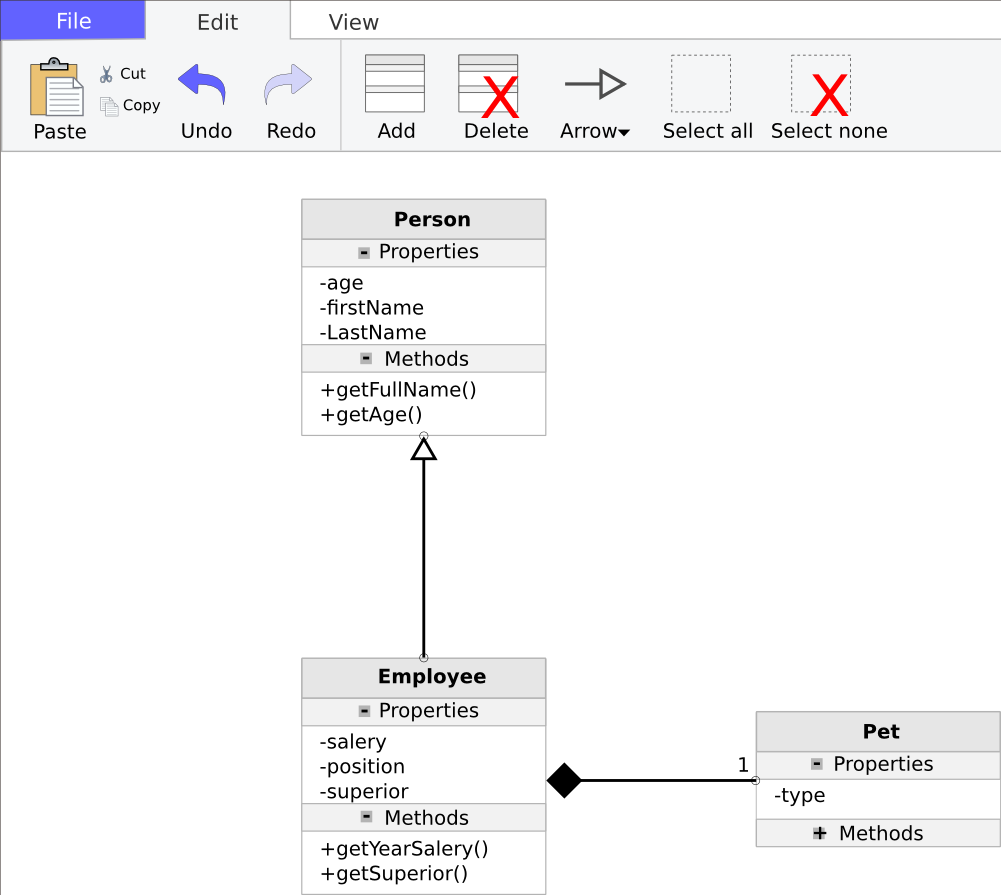
\includegraphics[width=\linewidth]{img/mockup}
\caption{Application mockup \label{mockup}}
\end{figure}

\newpage
\subsection{Requirements specification}
The specification is created using the \textit{MoSCoW} 
method\footnote{http://en.wikipedia.org/wiki/MoSCoW\_method}. Here, the 
requirements 
are divided in the following categories: \textit{Must}, \textit{should}, 
\textit{could} and \textit{won't}. This method can be seen as a combination of 
a requirements specification and an iteration plan, which helps the developers 
prioritize their work.

The application is a prototype and should not be considered as a final product 
but a basic concept ready for further development.

\begin{description}
	\item[Must have] \hfill \\
	\begin{enumerate}
		\item A graphical user interface supporting basic diagram editing 
		functionality
		\begin{itemize}
			\item Createing, editing and deleting classes
			\item Createing, editing and deleting relations
		\end{itemize}
		\item One diagram type
		\item DLL assembly containing the model for the diagram.
	\end{enumerate}
	\item[Should have] \hfill \\
	\begin{enumerate}
		\item Save/Open functionality
		\item Different relation types
		\item Undo/redo functionality
	\end{enumerate}
	\item[Could have] \hfill \\
	\begin{enumerate}
		\item Copy/cut/paste
		\item Export diagram as image
	\end{enumerate}
	\item[Won't have] \hfill \\
	\begin{enumerate}
		\item Multiple diagram types
		\item Advanced canvas functions
		\begin{itemize}
			\item Zoom
			\item Panning
		\end{itemize}
		\item Print funcionality
	\end{enumerate}
\end{description}





